\section{Resultados}\label{sec:resultados}

\subsection{\label{sub:data}Datos}\label{subsec:label{sub:data}datos}

\subsubsection{Primera parte}

Para comprobar el principio de Arqu�medes se toman 3 medidas.

Primero, el sistema cilindro hueco + cilindro macizo en al aire ($P_{vac}$).

Posteriormente, el mismo sistema con el cilindro macizo sumergido en el l�quido ($P_{ap}$).

Por �ltimo, se vierte el mismo l�quido en el cilindro hueco y se toma la medida con el cilindro macizo todav�a sumergido ($P_{ap} + P_{l\acute{\imath}q}$).

Las tablas~\ref{tab:c-1} y~\ref{tab:c-2} muestran las medidas obtenidas.

\begin{table}[h!]
    \caption{Cilindro macizo 1.}
    \label{tab:c-1}
    \begin{centering}
        \begin{tabular}{|P{40px}|P{37px}|P{37px}|P{65px}|}
            \hline
            L�quido   & $P_{vac}\,$(N) & $P_{ap}\,$(N) & $P_{ap} + P_{l\acute{\imath}q}\,$(N)  \\
            \hline
            \csvreader[late after line= \\, /csv/separator=semicolon ]{./files/data/c-1.csv}{}% use head of csv as column names
            {\csvcoli & \csvcolii      & \csvcoliii    & \csvcoliv}% specify your columns here
            \hline
        \end{tabular}
    \end{centering}
\end{table}

\begin{table}[h!]
    \caption{Cilindro macizo 2.}
    \label{tab:c-2}
    \begin{centering}
        \begin{tabular}{|P{40px}|P{37px}|P{37px}|P{65px}|}
            \hline
            L�quido   & $P_{vac}\,$(N) & $P_{ap}\,$(N) & $P_{ap} + P_{l\acute{\imath}q}\,$(N)  \\
            \hline
            \csvreader[late after line= \\, /csv/separator=semicolon ]{./files/data/c-2.csv}{}% use head of csv as column names
            {\csvcoli & \csvcolii      & \csvcoliii    & \csvcoliv}% specify your columns here
            \hline
        \end{tabular}
    \end{centering}
\end{table}

El principio de Arqu�medes afirma que $P_{vac}$ y $P_{ap} + P_{l\acute{\imath}q}$ deben ser iguales.

La precisi�n del dinam�metro es $\pm 0.01\,$N, por lo que las medidas obtenidas se encuentran dentro del rango esperado.

\subsubsection{Segunda parte}

En esta secci�n, se utiliza un soporte al que se van a�adiendo pesas de masa $m$.
La tabla~\ref{tab:2} muestra el peso en el vac�o $P_{vac}$ y el peso aparente con el soporte sumergido en agua $P_{agua}$ conforme se
va incrementando el n�mero de pesas $n$.

\begin{table}[h!]
    \caption{Pesos reales y aparentes en funci�n del n�mero de masas.}
    \label{tab:2}
    \begin{centering}
        \begin{tabular}{|P{20px}|P{41px}|P{41px}|P{77px}|}
            \hline
            $n$       & $P_{vac}\,$(N) & $P_{agua}\,$(N) & $(P_{vac} - P_{agua})\,$(N)           \\
            \hline
            \csvreader[late after line= \\, /csv/separator=semicolon ]{./files/data/2_es.csv}{}% use head of csv as column names
            {\csvcoli & \csvcolii      & \csvcoliii      & \csvcoliv}% specify your columns here
            \hline
        \end{tabular}
    \end{centering}
\end{table}


Las figuras~\ref{fig:p_vac} y~\ref{fig:p_agua} muestran $P_{vac}$ y $P_{agua}$ frente a $n$ respectivamente.
\footnote{En las figuras se emplea la notaci�n anglosajona, donde se utiliza el punto como separador de decimales.
}
Esto es equivalente a representar las ecuaciones~\ref{eq:masas_aire} y~\ref{eq:masas_agua}.

\begin{figure}[h!]
    \begin{center}
        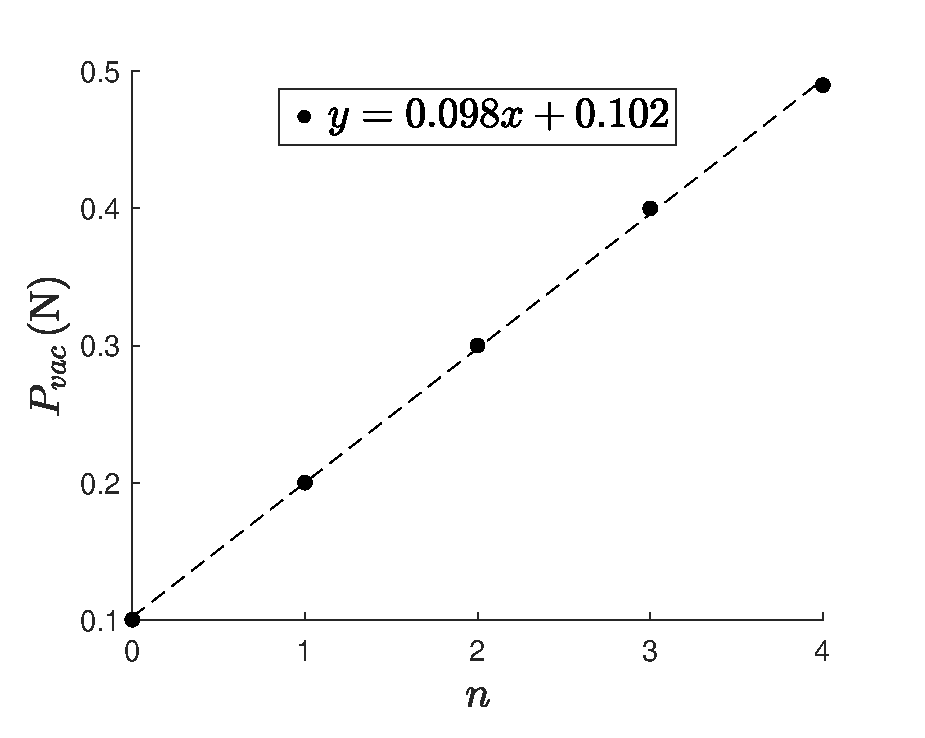
\includegraphics[width=0.8\columnwidth]{files/images/p_vac}
    \end{center}
    \caption{Peso en aire $P_{vac}$ frente al n�mero de pesas}
    \label{fig:p_vac}
\end{figure}

\begin{figure}[h!]
    \begin{center}
        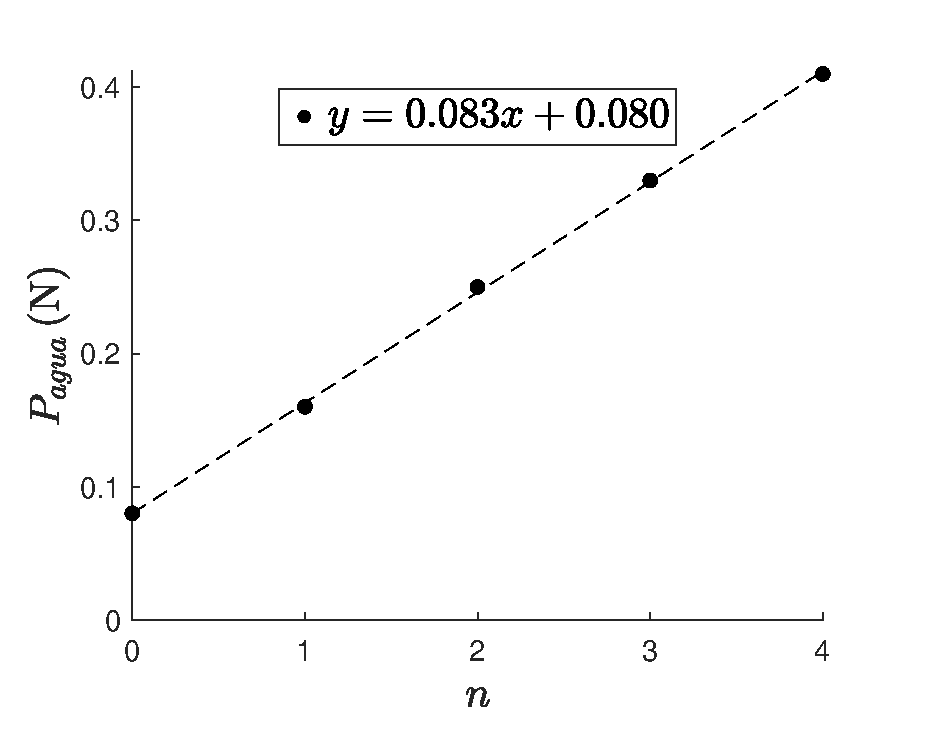
\includegraphics[width=0.8\columnwidth]{files/images/p_agua}
    \end{center}
    \caption{Peso aparente $P_{agua}$ frente al n�mero de pesas}
    \label{fig:p_agua}
\end{figure}

\FloatBarrier

Por �ltimo, la figura~\ref{fig:densidad} muestra $P_{vac}/(P_{vac} - P_{agua})$ frente a $n$.
Esta gr�fica representa la ecuaci�n~\ref{eq:d_s}.

\begin{figure}[h!]
    \begin{center}
        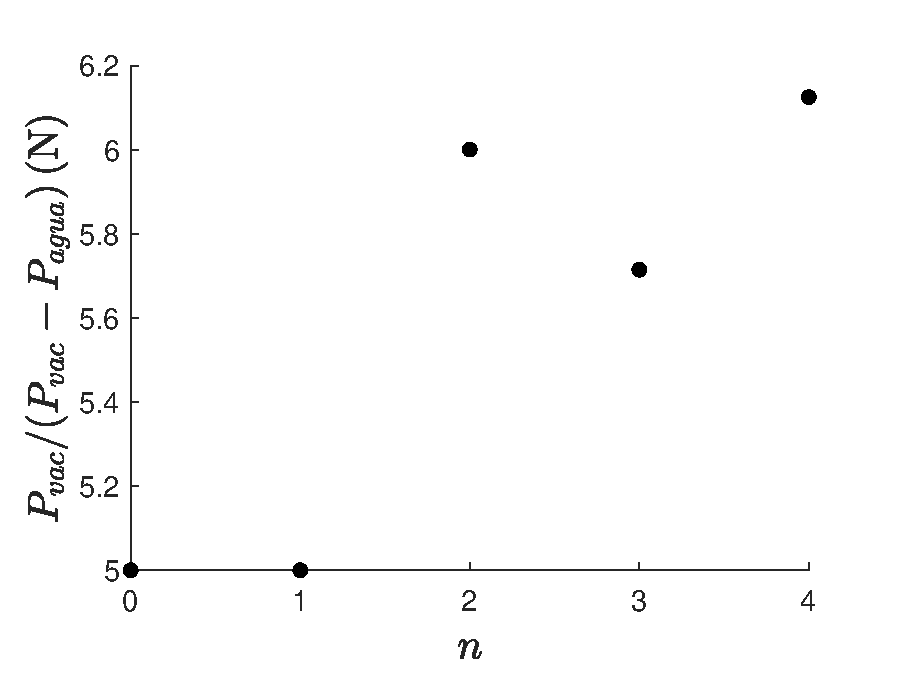
\includegraphics[width=0.8\columnwidth]{files/images/densidad}
    \end{center}
    \caption{$P_{vac}/(P_{vac} - P_{agua})$ frente al n�mero de pesas}
    \label{fig:densidad}
\end{figure}

\FloatBarrier

\subsection{\label{sub:results}An�lisis}\label{subsec:label{sub:results}analisis}

\subsubsection{}

Los valores de la pendiente $a$ y la ordenada en el origen $b$ de la recta de la gr�fica~\ref{fig:p_vac} con sus errores asociados son:
\begin{align*}
    a & = (0.0980 \pm 0.0012)\,\text{(N)}\\
    b & = (0.102 \pm 0.003)\,\text{(N)}\\
\end{align*}

La masa de las pesas es conocida, $m = 10\,$g.

De la ecuaci�n~\ref{eq:masas_aire}, sabemos que:
\begin{equation*}
    a = \rho_s \, V_s \, g
\end{equation*}

Como $m = \rho_s\, V_s$, despejamos $g$:
\begin{equation*}
    g = (9.80 \pm 0.12)\,\text{N/m$^2$}
\end{equation*}

A continuaci�n, utilizamos el valor obtenido de $g$ para estimar la masa del suspensor.

Tambi�n de la ecuaci�n~\ref{eq:masas_aire}, sabemos que:

\begin{equation*}
    b = m_{susp} \, g
\end{equation*}

Por tanto:
\begin{equation*}
    m_{susp} = (10.41 \pm 0.13)\,\text{g}
\end{equation*}

\subsubsection{\label{subsubsec:densidad_agua}}

Los valores de la pendiente $a'$ y la ordenada en el origen $b'$ de la recta de la gr�fica~\ref{fig:p_agua} con sus errores asociados son:
\begin{align*}
    a' & = (0.0830 \pm 0.0010)\,\text{(N)}\\
    b' & = (0.080 \pm 0.002)\,\text{(N)}\\
\end{align*}

De las ecuaciones~\ref{eq:masas_aire} y~\ref{eq:masas_agua} se tiene:
\begin{align*}
    \rho_{s} & = \frac{\rho_l}{1 - \frac{a'}{a}} \\
    \rho_{susp} & = \frac{\rho_l}{1 - \frac{b'}{b}}
\end{align*}

El error asociado a $\rho_s$ se puede calcular como:
\begin{equation*}
    \epsilon_{\rho_{s}} = \frac{\rho_l}{(1 - \frac{a'}{a})^2} \cdot \frac{1}{a} \cdot \Bigl(\frac{a'}{a}\epsilon_a + \epsilon_a' \Bigr)
\end{equation*}

Para $\rho_{susp}$, el error se calcula de modo similar.

Con todo ello, los valores de densidad de las pesas $\rho_s$ y del suspensor $\rho_{susp}$ son:

\begin{align*}
    \rho_s & = (6500 \pm 900)\,\text{kg/m$^3$} \\
    \rho_{susp} &= (4600 \pm 900)\,\text{kg/m$^3$}
\end{align*}

\subsubsection{}

En la figura~\ref{fig:densidad}, se observa que la densidad del sistema suspensor + pesas, aunque de manera irregular, parece aumentar con el n�mero de pesas.

Hemos mostrado en la secci�n~\ref{subsubsec:densidad_agua} que el suspensor es de un material m�s ligero que las pesas.

Si sigui�semos a�adiendo pesas, la curva tender�a asint�ticamente a una recta horizontal, cuya ordenada ser�a la densidad de las pesas.

\subsubsection{}

Utilizando los valores $P_{vac}$ y $P_{ap}$ de las tablas~\ref{tab:c-1} y~\ref{tab:c-2}, podemos calcular las densidades de
la glicerina y el vino.

\begin{table}[h!]
    \caption{Densidades de la glicerina y el vino.}
    \label{tab:densidades}
    \begin{centering}
        \begin{tabular}{|P{51px}|P{70px}|P{70px}|}
            \hline
            Cilindro  & $\rho_{glic}\,$(g/cm$^3$) & $\rho_{vin}\,$(g/cm$^3$)               \\
            \hline
            \csvreader[late after line= \\, /csv/separator=semicolon ]{./files/data/densidades.csv}{}% use head of csv as column names
            {\csvcoli & \csvcolii                 & \csvcoliii}% specify your columns here
            \hline
        \end{tabular}
    \end{centering}
\end{table}

Vemos en la tabla~\ref{tab:densidades} que el error asociado a las densidades es bastante grande, mayor que el $10 \%$.

La precisi�n del dinam�metro era $\pm 0.01\,$N, y la diferencia de las mediciones entre los l�quidos siempre est� dentro del margen
de error.

Esto, junto con el hecho de que el valor $g_{glic}$ deber�a ser mayor que $1\,$g/cm$^3$, nos sugiere que para obtener valores
de las densidades de los l�quidos m�s ajustados a la realidad, deber�amos haber utilizado un dinam�metro con mayor precisi�n.


